% !TeX root = ../../main.tex
% Hình: Pictures/Diagram/oracle-diagram.pdf (vector) và redis-diagram.png.
\subsection{Thiết kế cơ sở dữ liệu}\label{sec:intro-db-design}
\subsubsection{Mô hình dữ liệu trên Oracle}\label{sec:intro-db-oracle}
Oracle lưu trữ dữ liệu nghiệp vụ của ShopFlash thông qua 11 bảng chính, thuộc các nhóm quản lý người dùng, sản phẩm và tồn kho, giỏ hàng và đơn hàng, chương trình Flash Sale (Hình~\ref{fig:intro-oracle-model}).

% Sơ đồ vector khá dày chữ: cho rộng hơn vùng chữ 16 mm (8 mm mỗi bên) để vẫn đọc được khi in.
% Float [!hbp]: không cho lên đầu trang (sẽ đứng trước tiêu đề 1.4); không vừa thì sang trang float riêng.
\begin{figure}[!hbp]
\centering
\makebox[\linewidth][c]{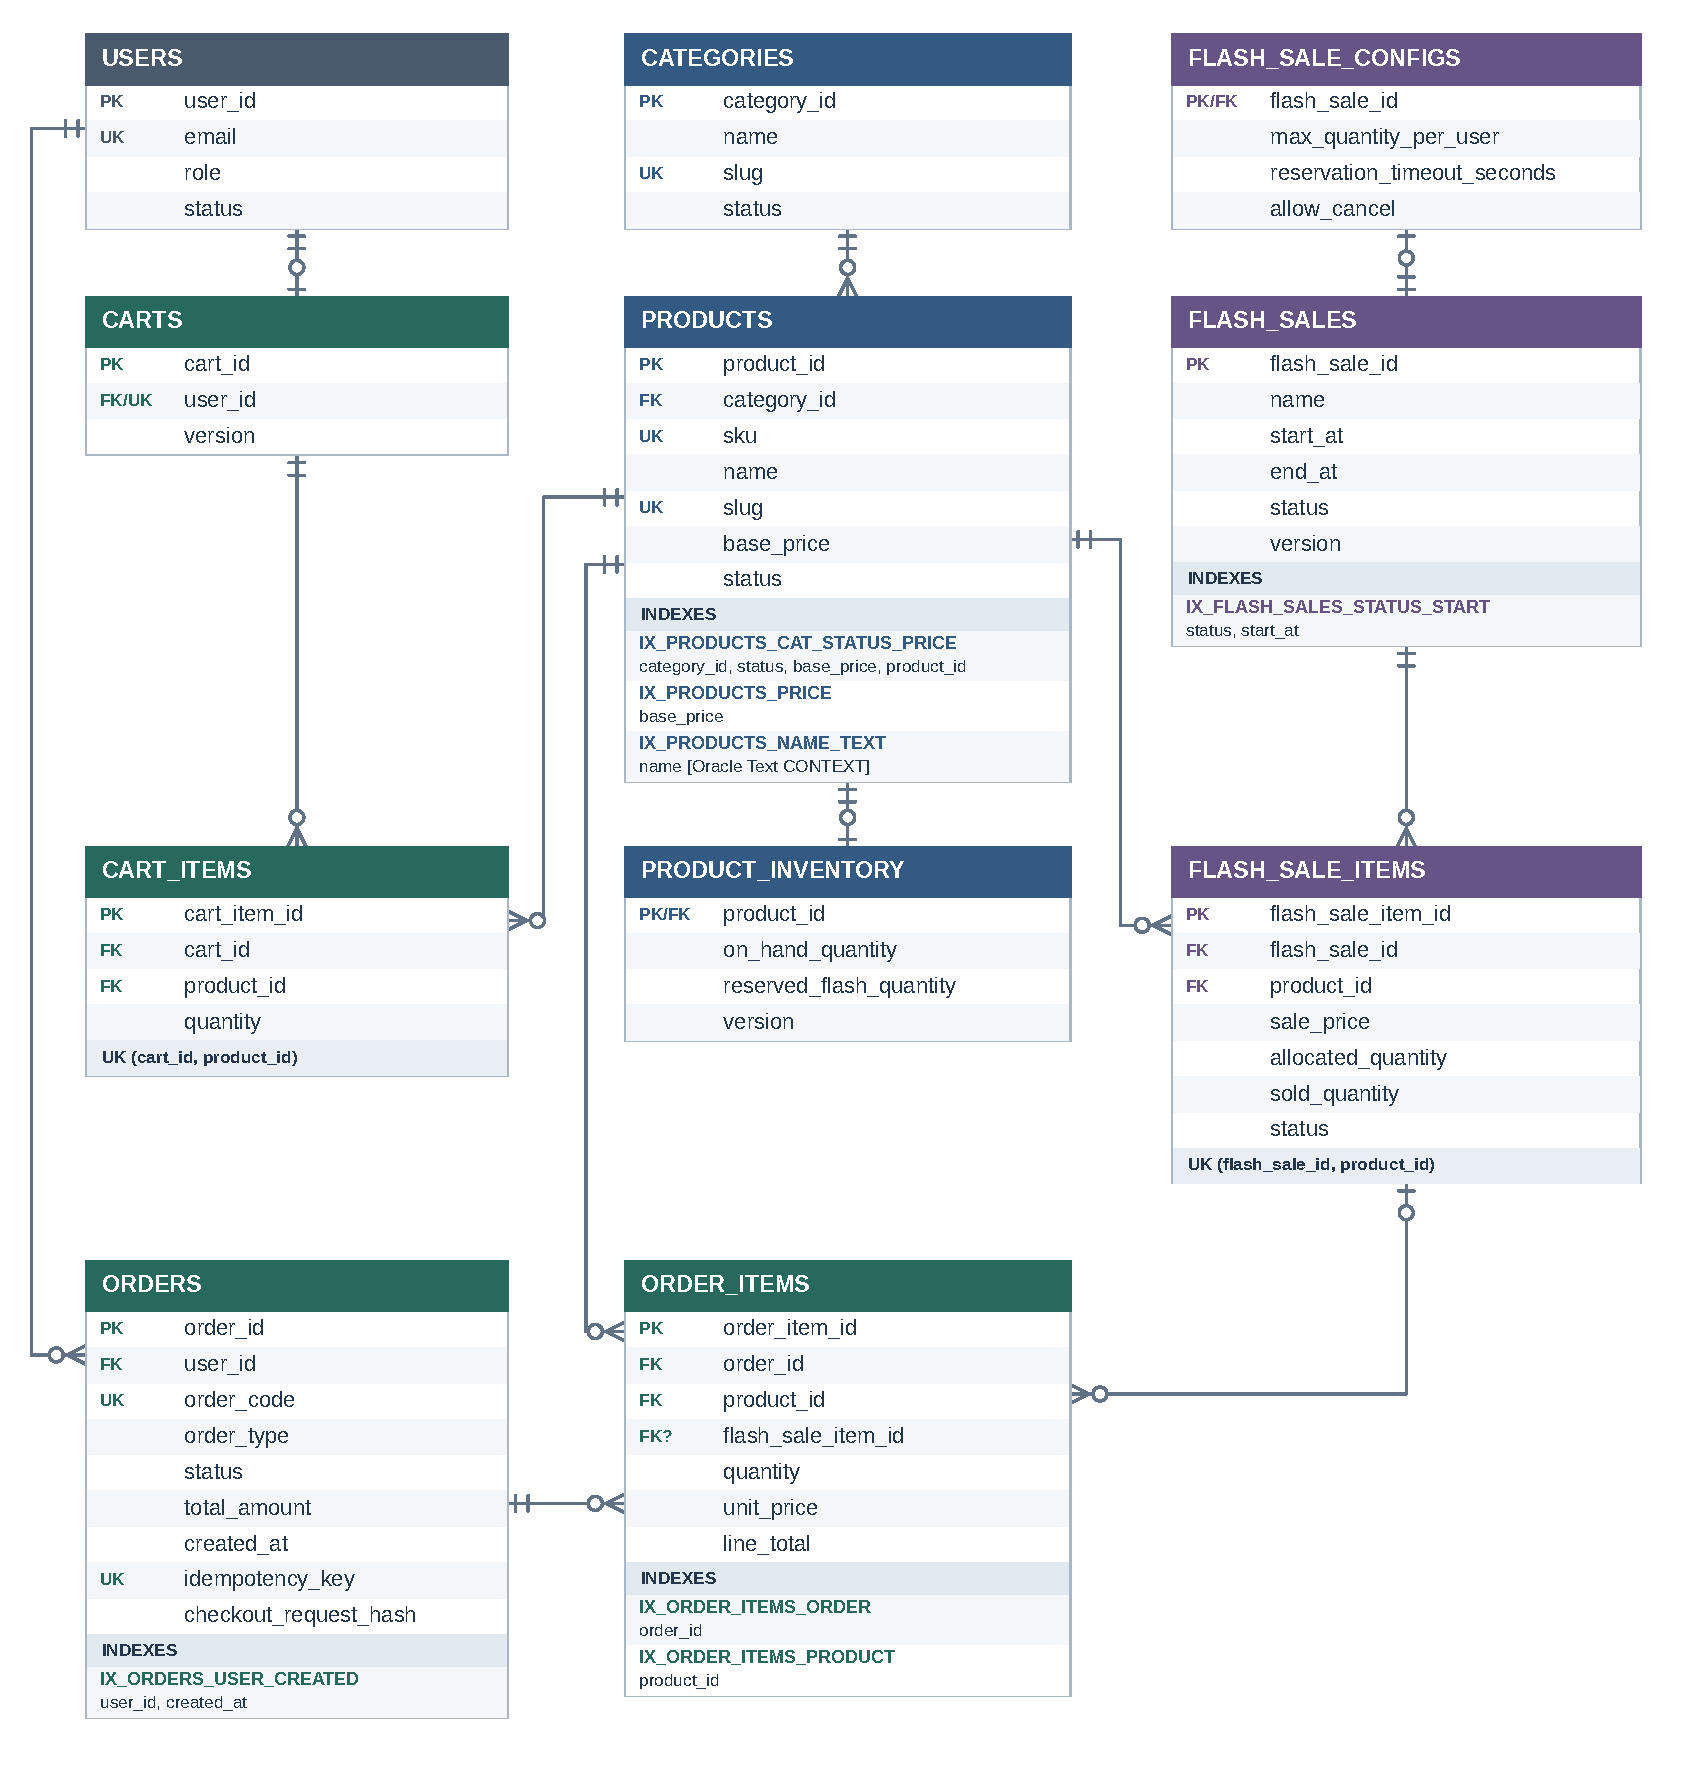
\includegraphics[width=176mm]{Pictures/Diagram/oracle-diagram.pdf}}
\caption{Sơ đồ mô hình dữ liệu quan hệ trên Oracle.}\label{fig:intro-oracle-model}
\end{figure}

% Bảng index đặt sớm trong mã nguồn để float nằm trong 1.4.1, không trôi qua tiêu đề 1.4.2.
\begin{table}[!htbp]
\centering
\caption{Các index bổ sung trên Oracle và mục đích sử dụng.}\label{tab:intro-oracle-index}
\reporttablesetup
\begin{tabularx}{\linewidth}{|>{\hsize=1.15\hsize\linewidth=\hsize\raggedright\arraybackslash\fontsize{10}{12}\selectfont\ttfamily}X|>{\hsize=0.8\hsize\linewidth=\hsize}L|>{\hsize=1.05\hsize\linewidth=\hsize}L|}
\hline
\rowcolor{ReportTableHead}
\normalfont\fontsize{11}{13}\selectfont\reportheader{Index} & \reportheader{Cột được lập chỉ mục} & \reportheader{Mục đích sử dụng} \\ \hline
IX\_PRODUCTS\_CAT\_STATUS\_PRICE & category\_id, status, base\_price, product\_id & Duyệt danh mục, lọc giá, sắp xếp và phân trang. \\ \hline
IX\_PRODUCTS\_PRICE & base\_price & Lọc sản phẩm theo giá trên toàn bộ cửa hàng. \\ \hline
IX\_PRODUCTS\_NAME\_TEXT & name & Tìm kiếm toàn văn dự phòng khi Redis không khả dụng. \\ \hline
IX\_ORDERS\_USER\_CREATED & user\_id, created\_at & Truy xuất lịch sử đơn hàng theo khách hàng và thời gian. \\ \hline
IX\_ORDER\_ITEMS\_ORDER & order\_id & Truy xuất các dòng hàng thuộc một đơn hàng. \\ \hline
IX\_ORDER\_ITEMS\_PRODUCT & product\_id & Hỗ trợ truy vấn thống kê và kiểm tra sản phẩm chưa bán. \\ \hline
IX\_FLASH\_SALES\_STATUS\_START & status, start\_at & Tìm các chương trình Flash Sale đến thời điểm kích hoạt. \\ \hline
\end{tabularx}
\end{table}

\paragraph*{Thiết kế các quan hệ và ràng buộc dữ liệu}

Bảng \texttt{PRODUCT\_INVENTORY} được tách khỏi \texttt{PRODUCTS} nhằm quản lý độc lập thông tin sản phẩm và trạng thái tồn kho. Số lượng tồn kho được phân biệt thành tổng số lượng hiện có (\texttt{on\_hand\_quantity}) và số lượng đã dành cho Flash Sale (\texttt{reserved\_flash\_quantity}). Tồn kho khả dụng cho mua hàng thông thường được xác định bằng hiệu của hai giá trị này.

Hai luồng mua hàng thông thường và Flash Sale sử dụng chung các bảng \texttt{ORDERS} và \texttt{ORDER\_ITEMS}. Trong đó, \texttt{order\_type} xác định loại đơn hàng, còn khóa ngoại \texttt{flash\_sale\_item\_id} trong \texttt{ORDER\_ITEMS} cho phép NULL đối với sản phẩm được mua theo hình thức thông thường. Thiết kế này giúp thống nhất việc lưu trữ và quản lý đơn hàng mà vẫn phân biệt được hai nghiệp vụ.

Các ràng buộc Primary Key, Foreign Key, Unique và Check được sử dụng để bảo đảm tính toàn vẹn dữ liệu. Một số ràng buộc còn phục vụ trực tiếp logic nghiệp vụ, chẳng hạn khóa duy nhất trên \texttt{CARTS.user\_id} bảo đảm mỗi người dùng có tối đa một giỏ hàng, trong khi \texttt{ORDERS.idempotency\_key} hỗ trợ ngăn tạo đơn hàng trùng lặp.

\paragraph*{Thiết kế chỉ mục (Index)}

Bên cạnh các index hỗ trợ khóa chính và ràng buộc duy nhất, hệ thống sử dụng một số index bổ sung dựa trên đặc điểm truy vấn của ứng dụng (Bảng~\ref{tab:intro-oracle-index}).

Đối với các truy vấn có nhiều điều kiện, hệ thống sử dụng index ghép (\emph{composite index}). Chẳng hạn, index trên danh mục, trạng thái và giá sản phẩm được tổ chức với các cột lọc theo giá trị xác định ở đầu, tiếp theo là cột lọc theo khoảng giá và sắp xếp. Cột \texttt{product\_id} ở cuối hỗ trợ xác định thứ tự ổn định khi nhiều sản phẩm có cùng giá.

Oracle Text được sử dụng như một phương án tìm kiếm dự phòng, cho phép ứng dụng tiếp tục phục vụ các yêu cầu tìm kiếm theo từ khóa khi RediSearch không khả dụng.

Sơ đồ chỉ thể hiện các index nghiệp vụ tiêu biểu. Việc lựa chọn index tại thời điểm thực thi phụ thuộc vào bộ tối ưu truy vấn của Oracle, thống kê dữ liệu và điều kiện truy vấn cụ thể.

\subsubsection{Mô hình dữ liệu trên Redis}\label{sec:intro-db-redis}
Redis không lưu trữ toàn bộ dữ liệu quan hệ của Oracle mà tổ chức dữ liệu theo các nhóm key phù hợp với nhu cầu truy vấn và xử lý của ứng dụng (Hình~\ref{fig:intro-redis-model}).

% Ảnh 1493×961 px có lề trắng hai bên; cắt theo vùng nội dung (266,45)–(1316,904) px, 1 px = 1 bp.
\begin{figure}[!htbp]
\centering
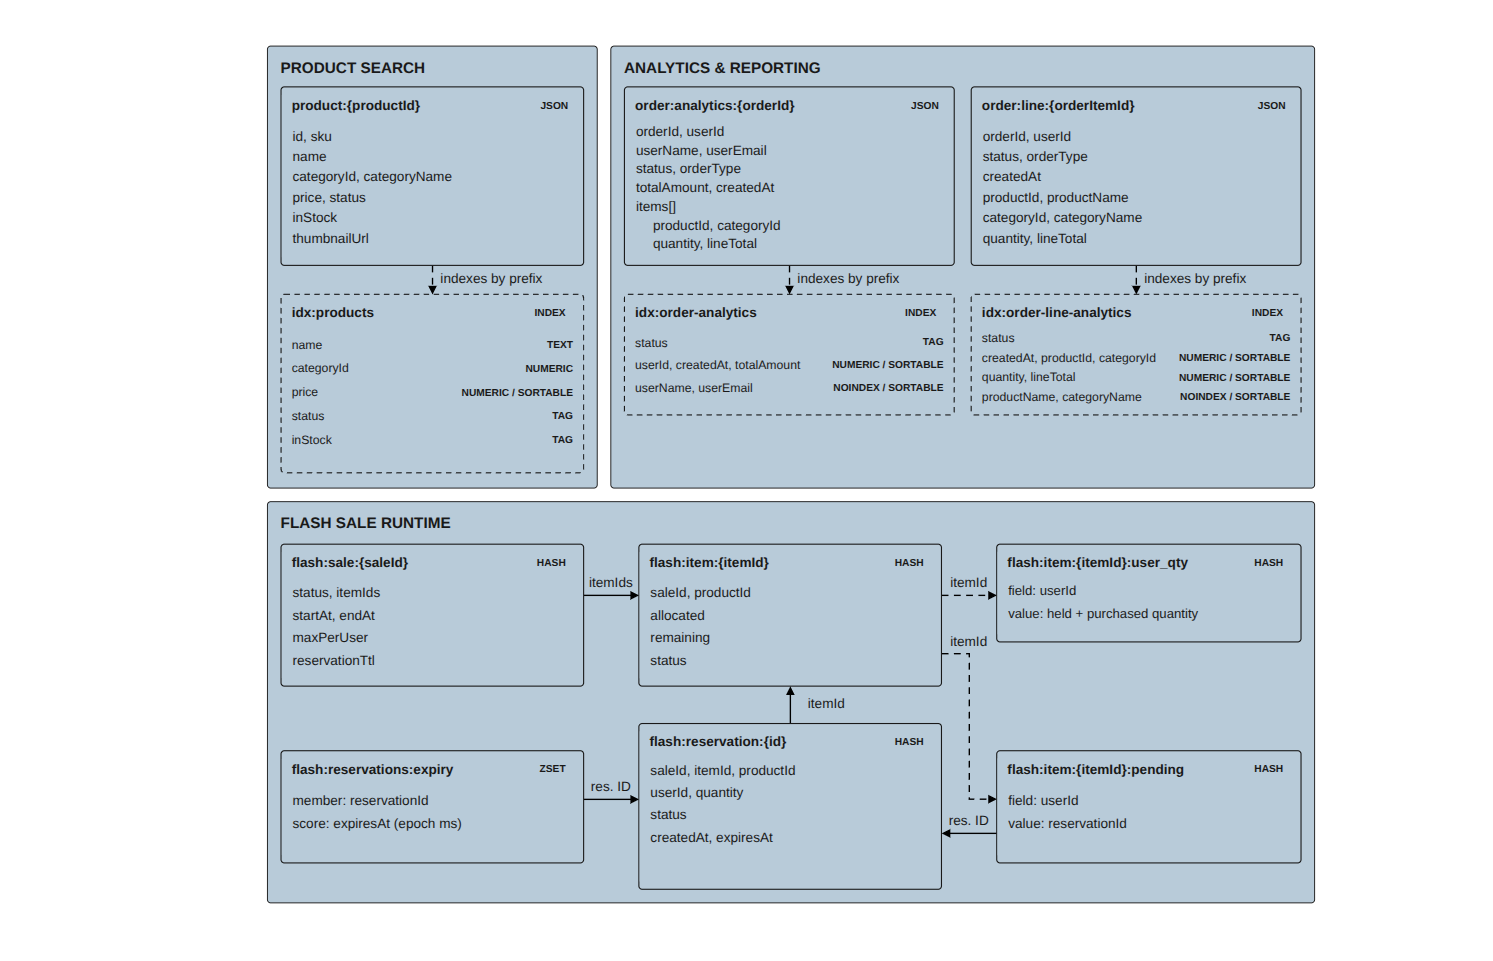
\includegraphics[width=\linewidth,trim={265bp 56bp 176bp 44bp},clip]{Pictures/Diagram/redis-diagram.png}
\caption{Mô hình tổ chức dữ liệu trên Redis.}\label{fig:intro-redis-model}
\end{figure}

\paragraph*{a. Product Search}

Thông tin sản phẩm được lưu dưới dạng JSON document, mỗi sản phẩm ứng với một key \texttt{product:\{productId\}}. Document tổng hợp dữ liệu từ ba bảng \texttt{PRODUCTS}, \texttt{CATEGORIES} và \texttt{PRODUCT\_INVENTORY} trên Oracle. Cách tổ chức này cho phép truy xuất trực tiếp thông tin sản phẩm, danh mục và trạng thái tồn kho mà không cần JOIN nhiều bảng.

Index \texttt{idx:products} được xây dựng trên các document sản phẩm, sử dụng các kiểu chỉ mục phù hợp với từng nhu cầu:

\begin{itemize}[leftmargin=1.3em,itemsep=2pt,topsep=3pt]
\item \texttt{TEXT}: tìm kiếm theo từ khóa trong tên sản phẩm.
\item \texttt{TAG}: lọc theo trạng thái sản phẩm và tình trạng còn hàng.
\item \texttt{NUMERIC}: lọc theo mã danh mục và khoảng giá.
\item \texttt{SORTABLE}: thuộc tính hỗ trợ sắp xếp theo giá.
\end{itemize}

\paragraph*{b. Order Analytics}

Dữ liệu thống kê được tổ chức thành hai loại JSON document:

\begin{itemize}[leftmargin=1.3em,itemsep=2pt,topsep=3pt]
\item \texttt{order:analytics:\{orderId\}}: lưu thông tin theo từng đơn hàng, phục vụ thống kê doanh thu và khách hàng.
\item \texttt{order:line:\{orderItemId\}}: lưu thông tin theo từng dòng hàng, phục vụ thống kê sản phẩm và danh mục.
\end{itemize}

Việc tách thành hai loại document giúp tổng hợp dữ liệu đúng cấp độ, tránh phải xử lý các mảng sản phẩm lồng nhau trong đơn hàng.

Hai index \texttt{idx:order-analytics} và \texttt{idx:order-line-analytics} hỗ trợ các phép nhóm và tổng hợp thông qua \texttt{FT.AGGREGATE}. Các trường thường xuyên được sử dụng trong quá trình tổng hợp được khai báo \texttt{SORTABLE} để hạn chế việc đọc lại toàn bộ document.

Thiết kế này chấp nhận lưu trữ một số thông tin trùng lặp nhằm giảm chi phí truy vấn tại thời điểm lập báo cáo.

\paragraph*{c. Flash Sale Runtime}

Dữ liệu Flash Sale được tổ chức thành các key phục vụ trực tiếp quá trình kiểm tra và giữ suất mua hàng (Bảng~\ref{tab:intro-flash-keys}).

% [H]: cuối Phần 1 có \clearpage, để float thì bảng bị dồn sang một trang riêng sau đoạn kết.
\begin{table}[H]
\centering
\caption{Các key Flash Sale runtime trên Redis.}\label{tab:intro-flash-keys}
\reporttablesetup
\begin{tabularx}{\linewidth}{|>{\hsize=1.25\hsize\linewidth=\hsize\raggedright\arraybackslash\fontsize{10}{12}\selectfont\ttfamily}X|>{\hsize=0.5\hsize\linewidth=\hsize}L|>{\hsize=1.25\hsize\linewidth=\hsize}L|}
\hline
\rowcolor{ReportTableHead}
\normalfont\fontsize{11}{13}\selectfont\reportheader{Key pattern} & \reportheader{Kiểu dữ liệu} & \reportheader{Vai trò} \\ \hline
flash:sale:\{saleId\} & Hash & Cấu hình và thời gian mở bán. \\ \hline
flash:item:\{itemId\} & Hash & Số lượng phân bổ và số suất còn lại. \\ \hline
flash:item:\{itemId\}:user\_qty & Hash & Theo dõi số lượng đã giữ hoặc mua của từng khách hàng. \\ \hline
flash:item:\{itemId\}:pending & Hash & Tra cứu reservation đang xử lý của từng khách hàng. \\ \hline
flash:reservation:\{id\} & Hash & Thông tin và trạng thái của lần giữ suất. \\ \hline
flash:reservations:expiry & Sorted Set & Quản lý reservation theo thời điểm hết hạn. \\ \hline
\end{tabularx}
\end{table}

Hash cho phép truy xuất và cập nhật từng trường dữ liệu độc lập, phù hợp với các thao tác kiểm tra quota, giới hạn mua và cập nhật trạng thái reservation. Sorted Set lưu reservation ID cùng thời điểm hết hạn dưới dạng score, giúp tìm các reservation đến hạn mà không cần quét toàn bộ keyspace.

Các key được phối hợp thông qua Lua Script để bảo đảm tính nguyên tử của thao tác giữ suất trên Redis.

Khác với Oracle, các liên kết trong sơ đồ Redis là tham chiếu logic do ứng dụng quản lý, không phải ràng buộc khóa ngoại được DBMS tự động thực thi.
